\section{Introduction}\label{sec:intro}

% ML doesn't work on atypical examples
Machine learning models are typically trained to minimize the average loss on a training set, with the goal of achieving high accuracy on an independent and identically distributed (i.i.d.) test set.
However, models that are highly accurate on average can still consistently fail on rare and atypical examples
\citep{hovy2015, blodgett2016, tatman2017, hashimoto2018repeated, duchi2019distributionally}.
Such models are problematic when they violate equity considerations \citep{jurgens2017, buolamwini2018gender}
or rely on \emph{spurious correlations}:
misleading heuristics that work for most training examples but do not always hold.
For example, in natural language inference (NLI)---%
determining if two sentences agree or contradict%
---the presence of negation words like `never' is strongly correlated with contradiction
due to artifacts in crowdsourced training data \citep{gururangan2018annotation, mccoy2019right}.
A model that learns this spurious correlation would be accurate on average on an i.i.d.\ test set but suffer high error on groups of data where the correlation does not hold
(e.g., the group of contradictory sentences with no negation words).

% DRO
To avoid learning models that rely on spurious correlations and therefore suffer high loss on some groups of data, we instead train models to minimize the \emph{worst-case} loss over groups in the training data.
The choice of how to group the training data allows us to use our prior knowledge of spurious correlations, e.g., by grouping together contradictory sentences with no negation words in the NLI example above.
This training procedure is an instance of distributionally robust optimization (DRO),
which optimizes for the worst-case loss over potential test distributions \citep{bental2013robust, duchi2016}.
Existing work on DRO has focused on models that cannot approach zero training loss, such as generative models \citep{oren2019drolm} or convex predictive models with limited capacity \citep{maurer2009empirical, shafieezadeh2015distributionally, namkoong2017variance,
duchi2018learning, hashimoto2018repeated}.

\begin{figure}[t!]
  \centering
  \vspace{-29mm}
  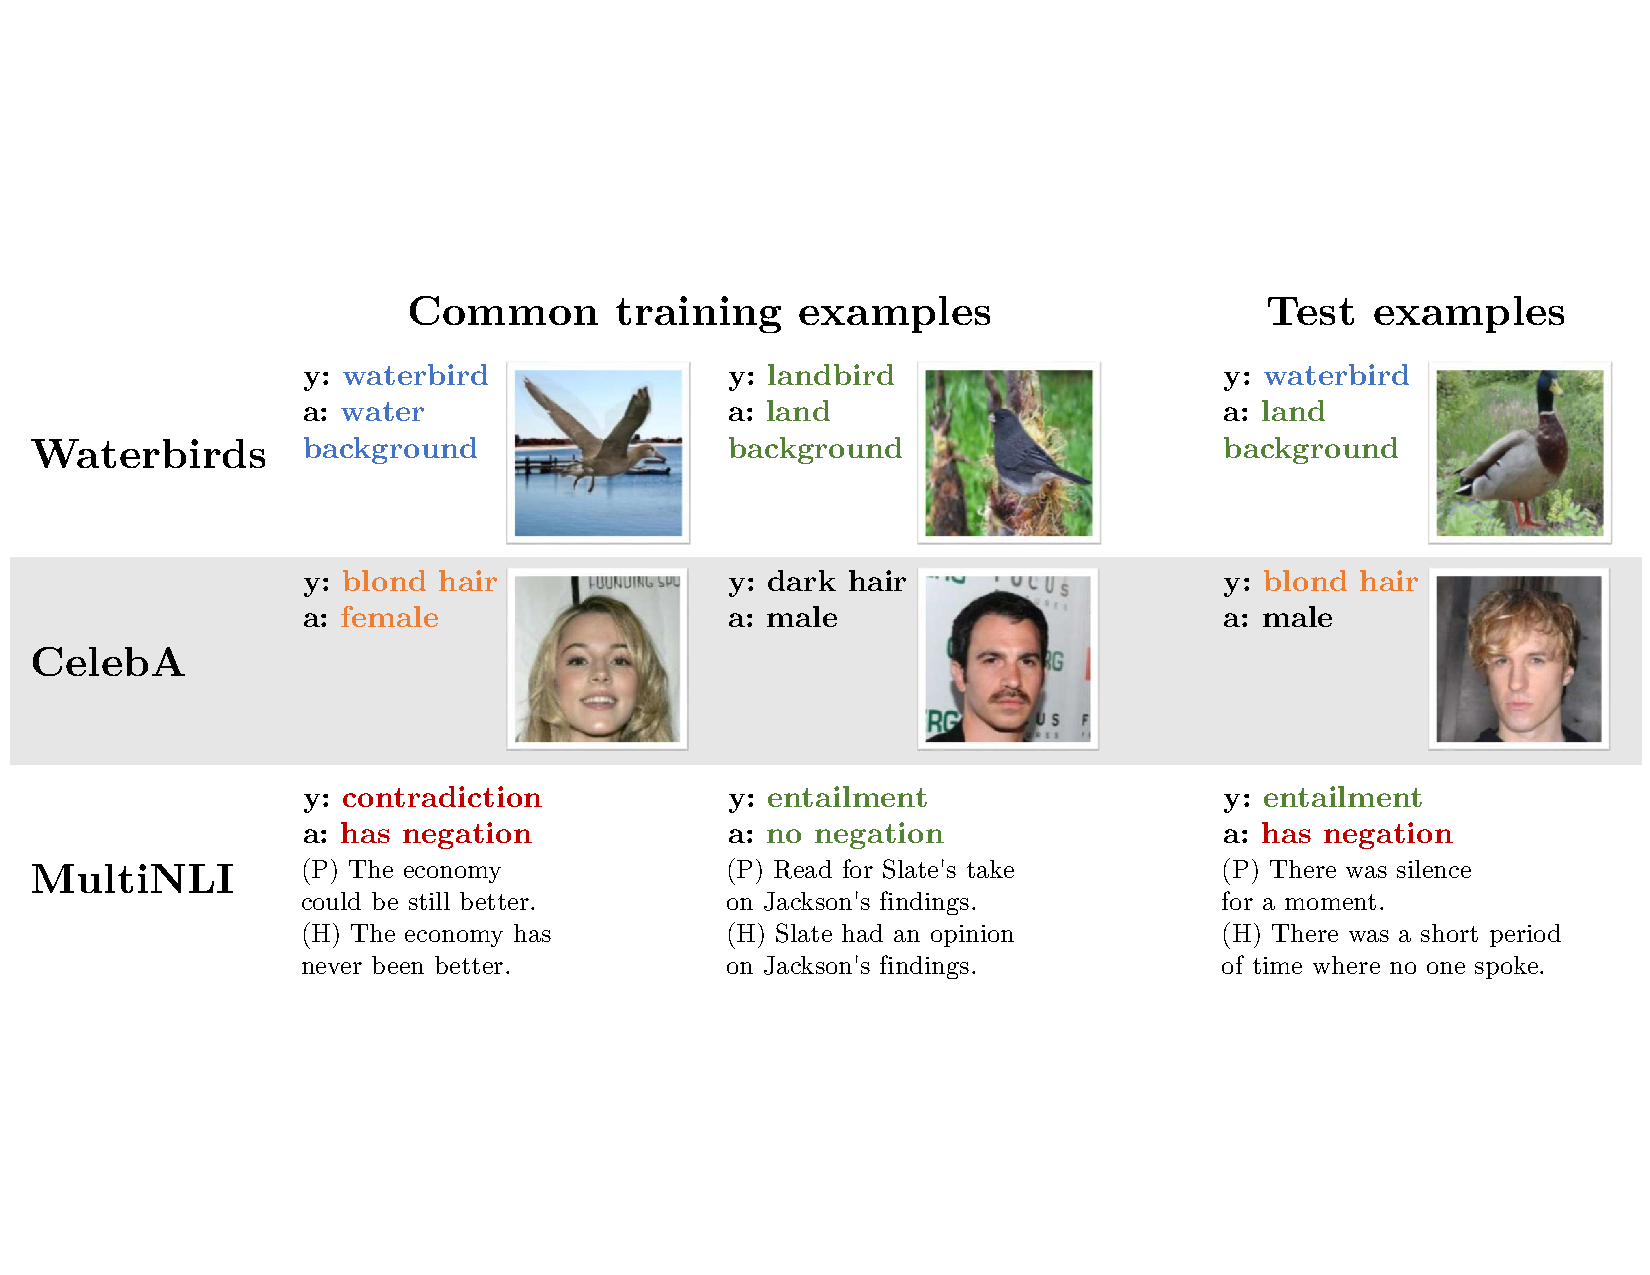
\includegraphics[scale=0.4]{figs/dataset.pdf}
  \caption{Representative training and test examples for the datasets we consider. The correlation between the label $y$ and the spurious attribute $a$ at training time does not hold at test time.}
  \vspace{-21mm}
  \label{fig:dataset}
\end{figure}

% Experiments (3 datasets), DRO doesn't work
We study group DRO in the context of overparameterized neural networks in three applications (\reffig{dataset})---%
natural language inference with the MultiNLI dataset \citep{williams2018broad},
facial attribute recognition with CelebA \citep{liu2015deep},
and bird photograph recognition with our modified version of the CUB dataset \citep{wah2011cub}.
The problem with applying DRO to overparameterized models is that if a model achieves zero training loss, then it is optimal on both the worst-case (DRO) and the average training objectives \citep{zhang2017understanding, wen2014robust}.
In the vanishing-training-loss regime,
we indeed find that group DRO models do no better than standard models trained to minimize average loss via empirical risk minimization (ERM):
both models have high average test accuracies and worst-group \emph{training} accuracies, but low worst-group \emph{test} accuracies (\refsec{experiments_unreg}).
In other words, the generalization gap is small on average but large for the worst group.

% Fix with regularization, group adjustments
In contrast, we show that strongly-regularized group DRO models that do not attain vanishing training loss can significantly outperform both regularized and unregularized ERM models.
We consider $\Ltwo$ penalties, early stopping (\refsec{experiments_complexity_control}),
and \emph{group adjustments} that minimize a risk measure which accounts
for the differences in generalization gaps between groups (\refsec{experiments_adjustments}).
Across the three applications, regularized group DRO improves worst-case test accuracies by 10--40 percentage points
while maintaining high average test accuracies.
These results give a new perspective on generalization in neural networks:
regularization might not be important for good average performance
(e.g., models can ``train longer and generalize better'' on average \citep{hoffer2017train}) but it appears important for good worst-case performance.

% Optimizer
Finally, to carry out the experiments, we introduce a new stochastic optimizer for group DRO
that is stable and scales to large models and datasets.
We derive convergence guarantees for our algorithm in the convex case and empirically show that it behaves well in our non-convex models (\refsec{alg}).
